\documentclass[11pt]{article}

\usepackage[T1]{fontenc}
\usepackage[utf8]{inputenc}
\usepackage{lmodern}
\usepackage{microtype}
\usepackage[a4paper,margin=28mm,headheight=14pt]{geometry}
\usepackage{amsmath,amssymb,amsthm,mathtools}
\usepackage{booktabs,tabularx,array,longtable}
\usepackage{enumitem}
\usepackage{xcolor}
\usepackage{listings}
\usepackage{graphicx}
\usepackage{fancyhdr}
\usepackage{hyperref}
\usepackage[nameinlink,noabbrev]{cleveref}

\definecolor{Navy}{HTML}{203864}
\definecolor{Blue}{HTML}{2F5597}
\definecolor{LightBlue}{HTML}{EAF2F8}
\definecolor{LightGray}{HTML}{F4F6F7}
\definecolor{DarkGray}{HTML}{4D5656}
\definecolor{Green}{HTML}{196F3D}
\definecolor{Red}{HTML}{A93226}

\hypersetup{
  colorlinks=true,
  linkcolor=Navy,
  citecolor=Green,
  urlcolor=Blue,
  pdftitle={W-Ranked Diagonal Hyperreflection: A Computable Contender 20 for BusyLean},
  pdfauthor={Research note prepared for Vladimir Reshetnikov}
}

\pagestyle{fancy}
\fancyhf{}
\lhead{W-Ranked Diagonal Hyperreflection}
\rhead{BusyLean Contender 20}
\cfoot{\thepage}

\newtheorem{theorem}{Theorem}[section]
\newtheorem{lemma}[theorem]{Lemma}
\newtheorem{proposition}[theorem]{Proposition}
\newtheorem{corollary}[theorem]{Corollary}
\theoremstyle{definition}
\newtheorem{definition}[theorem]{Definition}
\newtheorem{remark}[theorem]{Remark}

\newcommand{\Nat}{\mathbb{N}}
\newcommand{\Family}{\mathsf{Family}}
\newcommand{\Transformer}{\mathsf{Transformer}}
\newcommand{\Lift}{\mathsf{Lift}}
\newcommand{\WTree}{\mathsf{WTree}(\Nat)}
\newcommand{\code}[1]{\texttt{#1}}
\newcommand{\Cnineteen}{C_{19}}
\newcommand{\Ctwenty}{C_{20}}

\lstdefinelanguage{Lean}{
  morekeywords={def,theorem,lemma,abbrev,inductive,structure,namespace,end,open,
    import,where,match,with,fun,let,in,if,then,else,by,exact,apply,intro,
    have,show,change,rw,simpa,at,forall,exists,Prop,Type},
  sensitive=true,
  morecomment=[l]{--},
  morecomment=[s]{/-}{-/},
  morestring=[b]"
}
\lstset{
  language=Lean,
  basicstyle=\ttfamily\footnotesize,
  keywordstyle=\color{Navy}\bfseries,
  commentstyle=\color{Green},
  stringstyle=\color{Red},
  backgroundcolor=\color{LightGray},
  frame=single,
  rulecolor=\color{DarkGray},
  framesep=5pt,
  xleftmargin=0.5em,
  xrightmargin=0.5em,
  breaklines=true,
  breakatwhitespace=false,
  keepspaces=true,
  columns=fullflexible,
  showstringspaces=false,
  tabsize=2
}

\title{\textbf{W-Ranked Diagonal Hyperreflection}\\
\large A Computable Contender 20 for BusyLean}
\author{Research note prepared for Vladimir Reshetnikov}
\date{October 13, 2026}

\begin{document}
\maketitle

\begin{abstract}
The current BusyLean record, Contender 19, combines a large-Veblen-length
ladder of universes with a natural-number-indexed hierarchy of diagonal
transformer lifts.  This paper proposes and formally verifies a qualitative
extension: replace the finite rank by an arbitrary well-founded
\code{WTree Nat}.  At a rank-tree node, all child-rank lifts are spliced into
one lower lift; that lower lift both pre-amplifies the base transformer and
serves as the local lift while a fixed schedule is traversed.  The resulting
operation, \code{wDiagonalLift}, is structurally recursive and therefore
computable.

The new number is
\[
  \Ctwenty = F_{20}(F_{20}(42)),
\]
where \(F_{20}\) applies W-ranked hyperreflection to the large-Veblen ladder,
uses the entire Contender 19 construction as its oracle seed, and chooses both
its schedule and its W-valued rank by autonomous hyper-closures above the
Contender 19 schedule.  Lean proves the pointwise inequality
\[
  \operatorname{family}_{19}(n) < F_{20}(n)
\]
and, in particular, the required comparison
\[
  \Cnineteen < \Ctwenty.
\]
The checked development also proves strict parent-over-child rank growth and a
program domination theorem for every enumerated large-Veblen-ladder program at
the relevant depth.

The development was checked on Lean 4.34.0.  With Contender 19 precompiled, the
new definition phase took 0.84 seconds and the new comparison proof phase took
0.35 seconds on the recorded GitHub Actions runner.  The focused audit reports
only the repository-permitted axioms \code{propext} and \code{Quot.sound}; the
transitive closure of \code{contender\_20} avoids all earlier contender
constants.  No attempt is made to evaluate the numeral.
\end{abstract}

\tableofcontents
\newpage

\section{Problem statement and standard of success}

BusyLean is a formal version of the ``name the biggest number'' game: a
submission must define a closed natural number, must be computable in
principle, and must include a kernel-checked strict comparison with the
previous accepted contender.  Its rules additionally exclude
\code{noncomputable}, \code{partial}, \code{unsafe}, opaque stand-ins,
external implementations, and unapproved axioms.  A new contender should use
the previous \emph{construction}, rather than merely inserting the previous
constant into a trivial successor expression.

For this project, the formal success criterion is therefore not an informal
claim about a fast-growing hierarchy.  It is the existence of Lean terms
\begin{lstlisting}
def contender_20 : Nat := ...

theorem contender_19_lt_contender_20 :
  contender_19 < contender_20 := ...
\end{lstlisting}
that compile under the repository's pinned toolchain and pass its axiom and
dependency discipline.  The stronger goal pursued here is to make the new
construction qualitatively different from Contender 19, not merely to enlarge
an iteration parameter.

The exact formal claims established in the accompanying source are:
\begin{enumerate}[label=(\roman*),leftmargin=2.2em]
  \item W-ranked diagonal hyperreflection preserves progressivity;
  \item every W-rank is strictly inflationary over its base transformer;
  \item every visible child rank is strictly below its parent rank;
  \item Contender 19's entire family is pointwise below \(F_{20}\);
  \item every bounded large-Veblen-ladder program over the new seed is below
        \(F_{20}\);
  \item \(\Cnineteen < \Ctwenty\).
\end{enumerate}

\section{The audited baseline: Contender 19}

\subsection{The large-Veblen ladder}

Contender 19's reflected object language is a ladder of universes whose atoms
are large-Veblen terms.  In the repository implementation these are normal
Schuette-style bracket symbols: a constructor \(\varphi(A)\) carries a sorted
array of position--value pairs, and positions are themselves terms.  The
repository proves well-foundedness of the comparison and instantiates the
generic ladder normalization theorem with that well-founded atom order.

The numerical reflection operator is represented by a transformer
\code{lTransformer}.  Given a countable oracle family \(f_i\), the primitive
reflection value exceeds:
\begin{itemize}[leftmargin=2em]
  \item each visible oracle value \(f_i(n)\), for \(i\leq n\); and
  \item each enumerated, well-typed large-Veblen-ladder program of depth at
        most \(n\), run with the packed oracle family.
\end{itemize}
This is the core source of language strength inherited by the present work.

\subsection{Finite diagonal hyperreflection}

The generic amplifier used by Contender 19 is the finite hierarchy
\code{diagonalLift}.  In mathematical pseudocode, for a fixed schedule
\(S\in\WTree\),
\begin{align*}
  D_S(0)(B) &= \operatorname{liftTransformer}(B),\\
  D_S(k+1)(B) &=
    \operatorname{stageLift}\bigl(D_S(k),D_S(k)(B),S\bigr).
\end{align*}
Thus the rank-\(k\) lift occurs twice at successor rank: once as the local
lifting operation used throughout the schedule, and once as a pre-amplifier
of the base transformer.

Contender 19 chooses a self-fed finite rank and a self-fed autonomous schedule:
\begin{lstlisting}
def family18 (n : Nat) : Nat := F18 (F18 n)

def schedule19 (n : Nat) : WTree Nat :=
  Autonomous.realize
    (Autonomous.hyper (family18 n + 42)
      (Autonomous.encode tree12))

def rank19 (n : Nat) : Nat := family18 n + 1

def F19 (n : Nat) : Nat :=
  diagonalLift (schedule19 n) (rank19 n)
    lTransformer (fun _ => family18) n n

def contender_19 : Nat := F19 (F19 42)
\end{lstlisting}
This is already an extremely strong construction.  A successful successor
should not merely replace \code{rank19 n} by a larger natural number.

\section{The design gap: from finite rank to well-founded rank}

Natural-number rank is a genuine limitation in the \emph{shape} of the
amplifier.  No matter how enormous \(k\) is, \(D_S(k)\) is generated by a
single linear successor recursion.  The rank carries no branching data and no
limit structure.  By contrast, \(\WTree\) supports arbitrary countable
branching at every well-founded node.  It can therefore serve as executable
syntax for a transfinite recursion without introducing a nonconstructive
ordinal type or an oracle.

The key design question is how a node with countably many child ranks should
combine them.  A maximum is unavailable: the child objects are transformer
lifts, not numbers, and reflection is not monotone in its oracle.  The correct
operation is instead the same explicit-coordinate splice already used at the
transformer level.  Output coordinate \(i\) selects child \(i\).  This is
important: every growth proof can point to a concrete occurrence of a child,
rather than appeal to a false monotonicity principle.

The proposed jump is therefore:
\[
  \text{finite linear rank } k\in\Nat
  \quad\longrightarrow\quad
  \text{arbitrary well-founded rank } R\in\WTree.
\]
The object language remains the strongest language currently implemented in
BusyLean, so the new work isolates the improvement in the amplifier itself.

\section{Abstract transformer framework}

\subsection{Families, transformers, and lifts}

A BusyLean oracle family is extensionally a function
\[
  \Family = \Nat\to\Nat\to\Nat.
\]
The first argument is a family coordinate and the second is the numerical
input.  A transformer is a map between such families,
\[
  \Transformer = \Family\to\Family,
\]
and a transformer lift acts one type level higher,
\[
  \Lift = \Transformer\to\Transformer.
\]

A transformer \(T\) is \emph{progressive} when every visible seed coordinate
is strictly below every output coordinate at the same numerical input:
\[
  \operatorname{Progressive}(T) :\Longleftrightarrow
  \forall f,i,o,n,\ i\leq n \Rightarrow f(i,n)<T(f)(o,n).
\]
A lift \(L\) is \emph{strictly inflationary} when, for every progressive base
transformer \(T\),
\[
  T(f)(i,n)<L(T)(f)(o,n)
\]
for all visible \(i\leq n\) and all output coordinates \(o\).

\subsection{Why monotonicity is deliberately absent}

It would be tempting to order oracle families pointwise and prove reflection
monotone.  That statement is generally false: a reflected program may inspect
an oracle value and branch on it, so increasing the oracle can decrease the
program's result.  BusyLean's existing proofs correctly avoid this trap.
Every comparison follows an explicit occurrence of a seed value, a selected
child, or a selected transformer coordinate.

The W-ranked development follows the same discipline.  This makes its core
proofs robust and explains the apparently asymmetric use of output coordinate
\(0\) in splice operations.

\section{W-ranked diagonal hyperreflection}

\subsection{Splicing a family of lifts}

Given a countable family \(L_i\) of transformer lifts, define
\[
  \operatorname{spliceLifts}(L)(B)
  = \operatorname{spliceTransformers}\bigl(i\mapsto L_i(B)\bigr).
\]
The Lean definition is one line:
\begin{lstlisting}
def spliceLifts (lifts : Nat -> TransformerLift) :
    TransformerLift :=
  fun base => spliceTransformers (fun i => lifts i base)
\end{lstlisting}
At output coordinate \(i\), the resulting transformer runs the transformed
operator selected by \(i\), at that operator's canonical output coordinate
\(0\).

\begin{lemma}[Splice preservation]
If every \(L_i\) preserves progressivity, then
\(\operatorname{spliceLifts}(L)\) preserves progressivity.  If every \(L_i\)
is strictly inflationary, then the splice is strictly inflationary.
\end{lemma}

\begin{proof}[Proof idea]
For progressivity, output coordinate \(o\) selects \(L_o(B)\), and the assumed
progressivity of that transformed base supplies the inequality.  For strict
inflation, use the strictness theorem for \(L_o\) and its canonical output
coordinate \(0\).  No relation between distinct components is required.
\end{proof}

\subsection{The recursive definition}

Fix a local schedule \(S\in\WTree\).  The W-ranked hierarchy
\(W_S(R)\) is defined by structural recursion on the rank tree \(R\):
\begin{align*}
  W_S(\mathsf{leaf})
    &= \operatorname{liftTransformer},\\
  W_S(\mathsf{node}(f))(B)
    &= \operatorname{stageLift}(L,L(B),S),
\end{align*}
where
\[
  L=\operatorname{spliceLifts}\bigl(i\mapsto W_S(f(i))\bigr).
\]
In Lean:
\begin{lstlisting}
def wDiagonalLift (schedule : WTree Nat) :
    WTree Nat -> TransformerLift
  | .leaf => liftTransformer
  | .node f =>
      let lower : TransformerLift :=
        spliceLifts
          (fun i => wDiagonalLift schedule (f i))
      fun base =>
        stageLift lower (lower base) schedule
\end{lstlisting}

This is the exact W-tree analogue of one successor step of finite diagonal
hyperreflection.  All child-rank lifts are exposed through \code{lower}; then
\code{lower} occurs both intensionally in the pre-amplified base and
extensionally as the lift applied at every schedule node.

\subsection{Computability}

\begin{proposition}[Constructivity]
For every finite Lean value \(S,R:\code{WTree Nat}\), the term
\code{wDiagonalLift S R} is a computable transformer lift in the ordinary
operational semantics of Lean.
\end{proposition}

\begin{proof}
The only recursion defining \code{wDiagonalLift} is structural recursion on
\(R\).  The leaf branch returns an existing computable lift.  The node branch
forms ordinary Lean functions, uses the existing structural
\code{stageLift}, and recursively calls \code{wDiagonalLift} only on immediate
subtrees \(f(i)\).  No choice operator, unbounded search, partial definition,
unsafe code, opaque numerical stand-in, or external primitive occurs.
\end{proof}

The proposition says ``computable in principle,'' not ``feasible to
normalize.''  As with the earlier contenders, evaluating the final numeral is
both unnecessary and practically impossible.

\section{Formal growth theorems}

The accompanying file \code{TreeHyperReflectionFacts.lean} establishes three
central theorems.

\begin{theorem}[Progressivity at every W-rank]
For every schedule \(S\) and rank tree \(R\), the lift \(W_S(R)\) preserves
progressivity.
\end{theorem}

\begin{proof}[Induction structure]
At a leaf this is the existing theorem for \code{liftTransformer}.  At a node,
the induction hypotheses for all children imply progressivity of their splice.
That splice sends a progressive base to a progressive transformed base.  The
existing \code{stageLift\_progressive} theorem then closes the node case.
\end{proof}

\begin{theorem}[Strict inflation at every W-rank]
For every schedule \(S\) and rank tree \(R\), the lift \(W_S(R)\) is strictly
inflationary.
\end{theorem}

\begin{proof}[Induction structure]
The leaf case is the existing strictness theorem for autonomous lifting.  At a
node, let \(L\) be the splice of child-rank lifts.  By induction and the splice
lemmas, \(L\) preserves progressivity and is strictly inflationary.  Hence
\[
  B(f)(i,n)<L(B)(f)(i,n).
\]
The generic \code{base\_lt\_stageLift} theorem then gives
\[
  L(B)(f)(i,n)
  <\operatorname{stageLift}(L,L(B),S)(f)(o,n).
\]
Transitivity yields the result.
\end{proof}

\begin{theorem}[Child-rank strictness]
Let \(R=\mathsf{node}(f)\).  For every progressive base transformer \(B\), seed
family \(g\), and visible child coordinate \(i\leq n\),
\[
  W_S(f(i))(B)(g)(0,n)
  < W_S(R)(B)(g)(o,n)
\]
for every output coordinate \(o\).
\end{theorem}

\begin{proof}[Proof idea]
Coordinate \(i\) of the splice is definitionally the child transformer's
canonical output coordinate.  The parent stage strictly exceeds the spliced
lower transformer.  This identifies a concrete child occurrence and again
requires no monotonicity.
\end{proof}

Child-rank strictness is the formal reason the W-tree is not a decorative
parameter.  Moving from a visible child to its parent forces strict numerical
growth at the same input.

\section{Definition of Contender 20}

\subsection{Seed: the whole Contender 19 family}

Define
\begin{lstlisting}
def family19 (n : Nat) : Nat := F19 (F19 n)
\end{lstlisting}
so that \code{family19 42} unfolds to \code{contender\_19}.  This uses the
previous construction as a function of arbitrary input; it does not mention
the previous contender constant.

\subsection{A schedule and a W-valued rank}

The repository's \code{Autonomous} syntax supplies computable operations on
well-founded trees: encoding, realization, fixed-point-like closures, and
higher hyper-closures.  They are used here as transparent tree syntax, not as
a quotient with asserted ordinal identities.

First place a self-fed autonomous hyper-closure above Contender 19's schedule:
\begin{lstlisting}
def schedule20 (n : Nat) : WTree Nat :=
  Autonomous.realize
    (Autonomous.hyper (family19 n + 42)
      (Autonomous.encode (schedule19 n)))
\end{lstlisting}
Then place another such closure above the new schedule, retaining the result
as a tree rather than collapsing it to a natural-number rank:
\begin{lstlisting}
def rank20 (n : Nat) : WTree Nat :=
  Autonomous.realize
    (Autonomous.hyper (family19 n + 42)
      (Autonomous.encode (schedule20 n)))
\end{lstlisting}
The two roles are intentionally distinct.  \code{schedule20 n} controls the
operator-stage traversal at each rank node.  \code{rank20 n} controls the
transfinite shape of the hierarchy of lifts itself.

\subsection{The numerical function and final diagonal}

\begin{lstlisting}
def F20 (n : Nat) : Nat :=
  wDiagonalLift (schedule20 n) (rank20 n)
    lTransformer (fun _ => family19) n n

def contender_20 : Nat := F20 (F20 42)
\end{lstlisting}
Figure~\ref{fig:architecture} shows the dependency structure.

\begin{figure}[htbp]
  \centering
  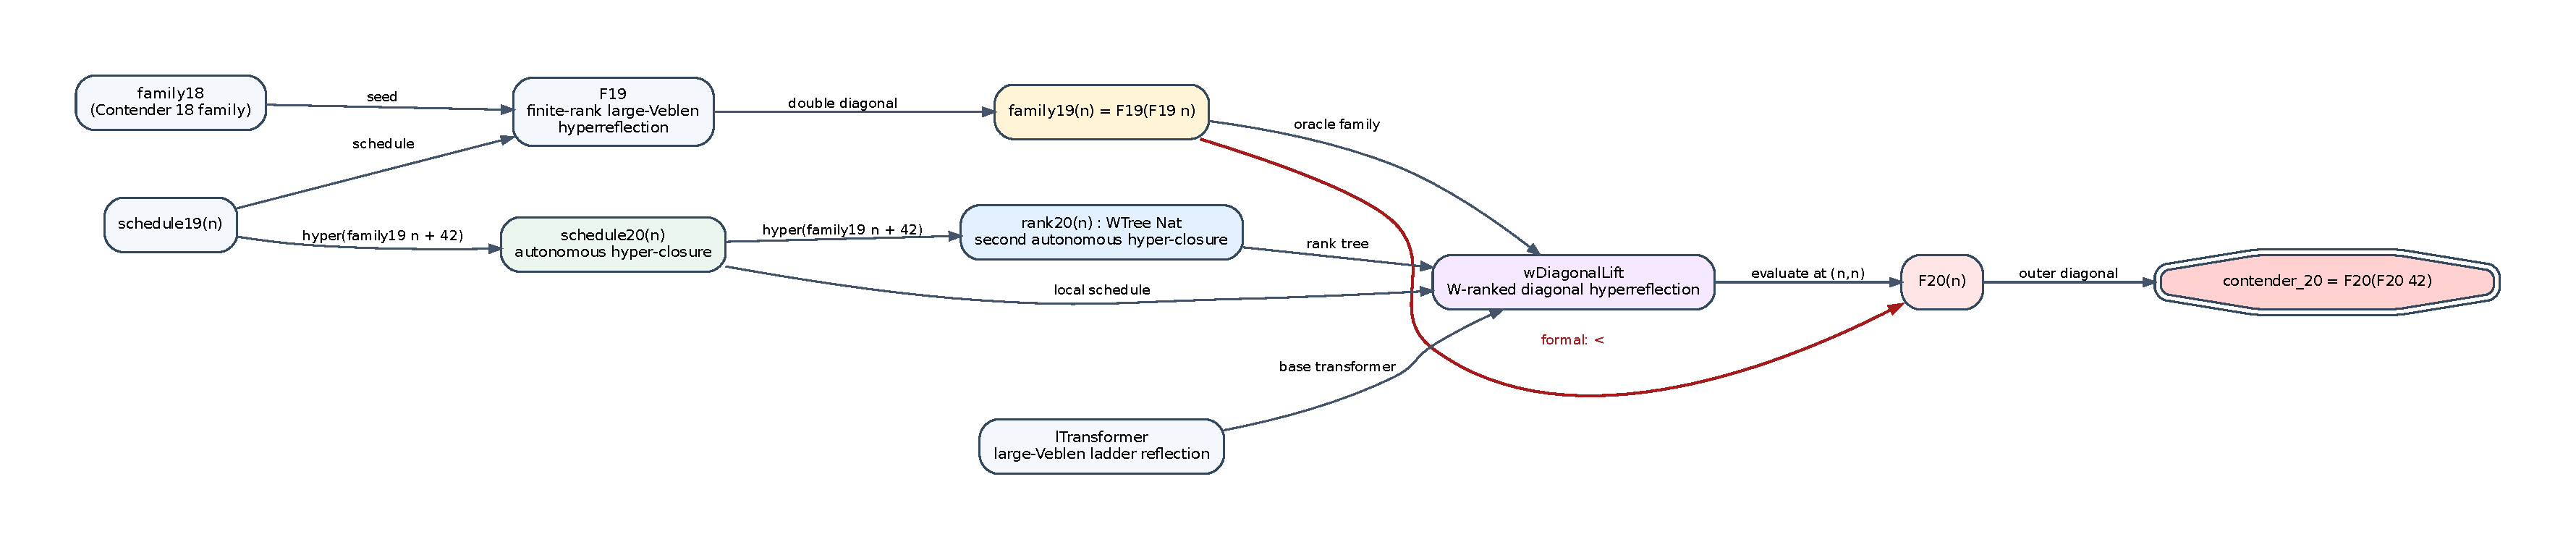
\includegraphics[width=\textwidth]{../figures/architecture.pdf}
  \caption{Construction of \code{contender\_20}.  The red edge is the central
  pointwise comparison proved in Lean.}
  \label{fig:architecture}
\end{figure}

\section{Dominance over Contender 19}

\subsection{Pointwise family domination}

\begin{theorem}[Checked in Lean]
For every \(n\in\Nat\),
\[
  \operatorname{family}_{19}(n)<F_{20}(n).
\]
\end{theorem}

\begin{proof}
The base transformer \code{lTransformer} is progressive.  By W-rank
progressivity, the transformed operator
\[
  W_{\operatorname{schedule}_{20}(n)}
    (\operatorname{rank}_{20}(n))(\code{lTransformer})
\]
is progressive.  Apply its progressivity to seed coordinate \(0\), output
coordinate \(n\), and input \(n\).  The seed family is constant in its first
coordinate, so seed coordinate \(0\) is exactly
\(\operatorname{family}_{19}(n)\).  The output is definitionally
\(F_{20}(n)\).
\end{proof}

This pointwise theorem is stronger and more reusable than a comparison only at
42.  It certifies that the new construction absorbs the whole previous family
at every input.

\subsection{Program domination}

Let \(t\) be an enumerated large-Veblen-ladder program of depth at most \(n\).
The primitive reflection theorem gives
\[
  \operatorname{lvalue}
    (\operatorname{packFamily}(\operatorname{family}_{19}),n,t)
  < \operatorname{reflectLFamily}
    (\operatorname{family}_{19},n).
\]
Strict inflation of the W-ranked lift then gives
\[
  \operatorname{reflectLFamily}
    (\operatorname{family}_{19},n)<F_{20}(n).
\]
Lean combines them as lvalue\_lt\_F20.  Thus the new number is not only
larger than the previous numerical seed; it also dominates every program in
the same bounded large-Veblen ladder when run over the stronger seed.

\subsection{The required comparison}

The final comparison is short because the general theorems carry the work:
\begin{lstlisting}
theorem contender_19_lt_contender_20 :
    contender_19 < contender_20 :=
  Nat.lt_trans (family19_lt_F20 42)
    (input_lt_F20 (F20 42))
\end{lstlisting}
Unfolding the definitions, the first inequality is
\[
  \Cnineteen=\operatorname{family}_{19}(42)<F_{20}(42),
\]
and the second is
\[
  F_{20}(42)<F_{20}(F_{20}(42))=\Ctwenty.
\]
Therefore \(\Cnineteen<\Ctwenty\), as required.

\section{Why the margin is structurally significant}

There are two distinct senses of ``larger'' in a formal large-number contest.
The first is the exact theorem \(\Cnineteen<\Ctwenty\).  The second is the
structural strength of the definition.  The present proposal improves both.

\subsection{Exact formal margin}

The following claims are kernel-checked, not heuristic:
\begin{itemize}[leftmargin=2em]
  \item the whole family \code{family19} is pointwise below \code{F20};
  \item every W-rank is strictly inflationary over the same base;
  \item every visible child rank is strictly below its parent;
  \item every bounded large-Veblen-ladder program over the new seed is below
        \code{F20};
  \item the final double diagonal strictly exceeds Contender 19.
\end{itemize}

\subsection{Heuristic growth calibration}

Any precise fast-growing-hierarchy calibration would require a semantic
analysis not present in BusyLean and not claimed here.  Nevertheless, the
construction supports a robust qualitative interpretation.

Finite \code{diagonalLift} iterates a rank-successor operation along
\(\Nat\).  Its self-fed rank may be inconceivably large, but its recursion
scheme is still finite and linear.  W-ranked hyperreflection instead permits
countable branching and well-founded limit structure in the \emph{rank of the
lift hierarchy itself}.  At a node, all child ranks remain separately
addressable through a splice, and the parent strictly exceeds every visible
child.  In ordinal-language shorthand, the change is analogous to replacing a
finite rank closure by a transfinite closure indexed by a concrete
well-founded tree.

The rank tree is not chosen near the bottom of the hierarchy.  It is a second
autonomous hyper-closure above a first new closure above Contender 19's own
schedule, and the hyper-iteration count is fed by \code{family19 n}.  This is
why the proposal should be regarded as a new amplifier level rather than a
parameter tweak.

The word ``analogous'' is essential.  The Lean theorem proves numerical
inequalities and recursion properties.  It does not identify the order type of
\code{rank20 n}, prove that the autonomous syntax realizes a specific named
ordinal, or equate \code{F20} with a standard fast-growing hierarchy.

\section{Rule compliance and audit}

\subsection{Closed, constructive natural number}

\code{contender\_20} has type \code{Nat} and is closed.  Every new recursive
definition is structural:
\begin{itemize}[leftmargin=2em]
  \item \code{wDiagonalLift} recurses on \code{WTree Nat};
  \item the inherited autonomous operations recurse on their inductive tree
        syntax or on \code{Nat};
  \item \code{F20} and \code{contender\_20} are ordinary total definitions.
\end{itemize}
The new files contain no \code{noncomputable}, \code{partial}, \code{unsafe},
\code{opaque}, \code{implemented\_by}, \code{extern}, custom axiom, or native
decision procedure.

\subsection{No direct dependence on prior constants}

A focused closure audit computes all constants reachable through the type and
value of \code{contender\_20}.  On the validated commit it reports:
\begin{lstlisting}[basicstyle=\ttfamily\small]
BusyLean.contender_20: closure of 4186 constants avoids all 15 forbidden names
\end{lstlisting}
where the forbidden list is \code{contender\_5} through
\code{contender\_19}.  The definition does use \code{F19} through
\code{family19}; this is precisely the permitted use of the previous
construction as a functional seed.

\subsection{Axiom report}

The focused audit reports:
\begin{center}
\begin{tabularx}{0.93\textwidth}{@{}lX@{}}
\toprule
Declaration & Reported axioms \\
\midrule
\code{spliceLifts} & none \\
\code{wDiagonalLift} and its generic growth theorems & \code{propext} \\
\code{family19}, \code{F20}, \code{contender\_20} & \code{propext}, \code{Quot.sound} \\
contender\_19\_lt\_contender\_20 & \code{propext}, \code{Quot.sound} \\
\bottomrule
\end{tabularx}
\end{center}
These are exactly within BusyLean's stated allowlist.  The appearance of
\code{Quot.sound} is inherited from the accepted normalization stack.

\section{Build validation and timing}

The attached receipt records a successful GitHub Actions run on Ubuntu 24.04
with Lean 4.34.0 and Lake 5.0.0.  The branch commit checked was
\begin{center}
\small\ttfamily af98b262699f4d19712682fc9a0cffe2ed353217
\end{center}

\begin{center}
\begin{tabular}{@{}lrr@{}}
\toprule
Phase & Wall time & Result \\
\midrule
Accepted base through \code{Comparison19} & 19.25 s & success \\
New definition modules through \code{Contender20} & 0.84 s & success \\
New proof module \code{Comparison20} & 0.35 s & success \\
Focused axiom and closure audit & 1.04 s (approximately) & success \\
\bottomrule
\end{tabular}
\end{center}

The repository's contest budget permits earlier accepted modules to be
precompiled.  Under that convention, the relevant new phases are 0.84 seconds
and 0.35 seconds, comfortably below the 15-second definition and 60-second
proof limits.  Timing depends on runner load and hardware, so the receipt is an
observed build record, not a universal bound.

\section{Repository integration}

The overlay consists of four library files and one focused audit:
\begin{longtable}{@{}>{\ttfamily\footnotesize\raggedright\arraybackslash}p{0.42\textwidth}p{0.52\textwidth}@{}}
\toprule
Path & Purpose \\
\midrule
\endfirsthead
\toprule
Path & Purpose \\
\midrule
\endhead
BusyLean/TreeHyperReflection.lean & Defines \code{spliceLifts} and \code{wDiagonalLift}. \\
BusyLean/TreeHyperReflectionFacts.lean & Proves progressivity, strict inflation, and child-rank strictness. \\
BusyLean/Contender20.lean & Defines \code{family19}, \code{schedule20}, \code{rank20}, \code{F20}, and \code{contender\_20}. \\
BusyLean/Comparison20.lean & Proves pointwise, program, and final contender comparisons. \\
test/Contender20Audit.lean & Prints axioms, checks the forbidden-constant closure, and verifies theorem signatures. \\
\bottomrule
\end{longtable}

After copying the files into a checkout at the audited base commit, append the
four module imports to \code{BusyLean.lean}.  Then run:
\begin{lstlisting}[language=bash]
lake build BusyLean.Contender20
lake build BusyLean.Comparison20
lake env lean test/Contender20Audit.lean
\end{lstlisting}
The archive includes an integration patch and detailed instructions.

\section{Limitations and research integrity}

\begin{enumerate}[leftmargin=2.2em]
  \item \textbf{No numerical evaluation.}  The final natural number is
  executable in principle but not practically evaluable.  The development
  checks its definition and comparison without reducing it.

  \item \textbf{No exact ordinal assignment.}  The words ``large Veblen,''
  ``autonomous,'' and ``hyper-closure'' describe repository syntax and its
  intended proof-theoretic motivation.  This work does not prove an isomorphism
  with a canonical ordinal notation system or identify the exact order type of
  \code{rank20}.

  \item \textbf{Strict dominance is exact; the size calibration is not.}
  The theorem \(\Cnineteen<\Ctwenty\) and the pointwise family theorem are
  formal.  Statements about exponentiation, fixed points, or transfinite
  hierarchy levels are explanatory heuristics unless explicitly represented
  by a Lean theorem.

  \item \textbf{The W-rank is external syntax.}  The rank tree is constructed
  in Lean from autonomous tree operations.  A still stronger direction would
  let the reflected object language generate and inspect its own rank trees,
  followed by a normalization proof for that enriched language.
\end{enumerate}

\section{Further research questions}

\begin{enumerate}[leftmargin=2.2em]
  \item \textbf{Finite-rank embedding.}  Define a canonical embedding of the
  existing natural-rank hierarchy \code{diagonalLift} into
  \code{wDiagonalLift} and prove an explicit domination theorem at every finite
  rank, not merely strict parent-over-child growth.

  \item \textbf{Rank monotonicity under tree embedding.}  Identify a
  simulation relation \(R\preccurlyeq R'\) between rank trees strong enough to
  prove \(W_S(R)\) below \(W_S(R')\) without assuming oracle monotonicity.
  The likely formulation must carry explicit coordinate witnesses.

  \item \textbf{Generic well-founded rank types.}  Replace \code{WTree Nat}
  by an arbitrary inductive well-founded branching signature and prove the
  amplifier theorems once, parametrically.

  \item \textbf{Self-generated rank trees.}  Extend the large-Veblen ladder
  language with a safe tree datatype and recursor, then make the rank range over
  every tree generated by the language itself.  The challenge is to retain a
  transparent strong-normalization proof.

  \item \textbf{Semantic ordinal calibration.}  Construct an ordinal
  interpretation for the transformer-lift hierarchy and prove upper and lower
  bounds for finite and W-ranked hyperreflection.  Even a coarse sandwich
  theorem would turn the present heuristic comparison into a mathematical
  classification.

  \item \textbf{Reflection over rank-indexed languages.}  Let each rank node
  select not only a lift but also a stronger universe ladder or atom notation
  system.  This would combine transfinite amplifier rank with transfinite
  language strength rather than holding the language fixed.

  \item \textbf{Independent kernel checking.}  Add \code{leanchecker} and
  \code{nanoda} jobs, subject to their support for Lean 4.34.0 and the project's
  axiom policy, to supplement the standard Lean kernel build.

  \item \textbf{Machine-checked budget harness.}  Extend
  \code{scripts/check.py} so Contender 20's definition and proof phases are
  timed separately, the closure audit is mandatory, and a signed or hashed
  receipt is emitted automatically.
\end{enumerate}

\section{Conclusion}

The proposed Contender 20 makes a specific qualitative move: the rank of
BusyLean's strongest generic amplifier is promoted from a natural number to an
arbitrary well-founded, countably branching tree.  The node operation is not a
metaphorical limit.  It explicitly splices all child-rank lifts, uses the
splice to amplify the base, and traverses the local schedule with the same
lower-rank lift.  Lean proves that every rank is progressive and strictly
inflationary and that each visible child rank is strictly below its parent.

Instantiating this amplifier with the large-Veblen ladder, seeding it with the
whole Contender 19 family, and choosing a self-fed autonomous W-rank yields a
closed computable natural number.  The checked theorem
\[
  \boxed{\Cnineteen<\Ctwenty}
\]
meets the contest's exact success criterion, while the W-valued rank supplies a
substantial structural margin beyond the previous finite-rank construction.

\appendix

\section{Lean theorem inventory}

The main declarations checked in the package are:
\begin{longtable}{@{}>{\ttfamily\footnotesize\raggedright\arraybackslash}p{0.46\textwidth}p{0.48\textwidth}@{}}
\toprule
Declaration & Content \\
\midrule
\endfirsthead
\toprule
Declaration & Content \\
\midrule
\endhead
spliceLifts\_preservesProgressive & A splice of progressivity-preserving lifts preserves progressivity. \\
spliceLifts\_strictlyInflationary & A splice of strictly inflationary lifts is strictly inflationary. \\
wDiagonalLift\_preservesProgressive & Every W-ranked lift preserves progressivity. \\
wDiagonalLift\_strictlyInflationary & Every W-ranked lift strictly exceeds its base transformer. \\
wDiagonalLift\_child\_lt & Every visible child-rank output is strictly below the parent-rank output. \\
family19\_lt\_F20 & \(\operatorname{family}_{19}(n)<F_{20}(n)\) for every \(n\). \\
raw\_reflection\_lt\_F20 & One raw large-Veblen reflection over the new seed is below \(F_{20}(n)\). \\
\code{lvalue\_lt\_F20} & Every enumerated bounded large-Veblen-ladder program over the new seed is below \(F_{20}(n)\). \\
F19\_lt\_F20 & \(F_{19}(n)<F_{20}(n)\) for every \(n\). \\
input\_lt\_F20 & \(n<F_{20}(n)\) for every \(n\). \\
\code{contender\_19\_lt\_contender\_20} & The required strict comparison. \\
\bottomrule
\end{longtable}

\section{Core source excerpt}

\begin{lstlisting}
def spliceLifts (lifts : Nat -> TransformerLift) :
    TransformerLift :=
  fun base => spliceTransformers (fun i => lifts i base)

def wDiagonalLift (schedule : WTree Nat) :
    WTree Nat -> TransformerLift
  | .leaf => liftTransformer
  | .node f =>
      let lower : TransformerLift :=
        spliceLifts
          (fun i => wDiagonalLift schedule (f i))
      fun base =>
        stageLift lower (lower base) schedule

def family19 (n : Nat) : Nat := F19 (F19 n)

def schedule20 (n : Nat) : WTree Nat :=
  Autonomous.realize
    (Autonomous.hyper (family19 n + 42)
      (Autonomous.encode (schedule19 n)))

def rank20 (n : Nat) : WTree Nat :=
  Autonomous.realize
    (Autonomous.hyper (family19 n + 42)
      (Autonomous.encode (schedule20 n)))

def F20 (n : Nat) : Nat :=
  wDiagonalLift (schedule20 n) (rank20 n)
    lTransformer (fun _ => family19) n n

def contender_20 : Nat := F20 (F20 42)
\end{lstlisting}

\section{Validation receipt summary}

\begin{verbatim}
commit: af98b262699f4d19712682fc9a0cffe2ed353217
Lean 4.34.0, Lake 5.0.0
accepted base: 19.25 s
definition phase: 0.84 s
proof phase: 0.35 s
contender_20 closure: 4186 constants; avoids 15 forbidden names
required theorem: contender_19 < contender_20
\end{verbatim}
The archive contains the complete machine-generated \code{validation-ci.log}.

\begin{thebibliography}{99}

\bibitem{aaronson}
Scott Aaronson.
\newblock \emph{Who Can Name the Bigger Number?}
\newblock Online essay, 1999.

\bibitem{roux}
Cody Roux.
\newblock \emph{name-the-biggest-number}.
\newblock Coq contest repository, GitHub.

\bibitem{busyLean}
Vladimir Reshetnikov.
\newblock \emph{BusyLean: name the biggest number, in Lean}.
\newblock GitHub repository, audited at commit
\code{64d31a0cf6f1aa4477a088be5554957de6e87a61}, October 13, 2026.

\bibitem{lean4}
Leonardo de Moura and Sebastian Ullrich.
\newblock The Lean 4 theorem prover and programming language.
\newblock In \emph{Automated Deduction -- CADE 28}, Lecture Notes in Computer
Science 12699, pages 625--635. Springer, 2021.

\bibitem{girard}
Jean-Yves Girard, Paul Taylor, and Yves Lafont.
\newblock \emph{Proofs and Types}.
\newblock Cambridge Tracts in Theoretical Computer Science 7. Cambridge
University Press, 1989.

\bibitem{schuette}
Kurt Schuette.
\newblock \emph{Proof Theory}.
\newblock Grundlehren der mathematischen Wissenschaften 225. Springer, 1977.

\bibitem{pohlers}
Wolfram Pohlers.
\newblock \emph{Proof Theory: The First Step into Impredicativity}.
\newblock Universitext. Springer, 2009.

\bibitem{moerdijk}
Ieke Moerdijk and Erik Palmgren.
\newblock Wellfounded trees in categories.
\newblock \emph{Annals of Pure and Applied Logic}, 104(1--3):189--218, 2000.

\end{thebibliography}

\end{document}
